
\chapter{Hynesim}
\label{chap:hynesim}

Firstly, I will present Hynesim. In fact, I will use this tool to create our network and test our solution so it is
important to introduce it.

\section{Presentation}

\begin{figure}[h]
  \centering
  
\includegraphics[width=0.5\textwidth]{hynesim}
  \caption{Hynesim logo}
  \label{fig:hynesim}
\end{figure}


\definition{Hynesim}{Means HYbrid NEtwork SIMulation, is a distribution platform of simulation of information
  systems developed by Diateam. \cite{hynesim}}

The platform was initially developed by Diateam for DGA\footnote{French Procurement Agency} MI (Maitrise de
l'information) to create virtual networks. But now is a major project to develop information systems and automatize
cyber security attacks. This project has two version, an open source version and a professional version. The open
source version has less options, but I will use this version for this project.

\section{Architecture}

In order to work, Hynesim needs a server with on it the main software. This software is the virtualization part. It
manages virtual machines and networks.

Moreover, to see virtual machine and interact with them, users needed to have a client interface. This interface
can be installed on a simple computer.

To add a virtual machine to Hynesim, I need to create it on Virtual Box\footnote{More information here:
  \url{https://www.virtualbox.org/}} or VMWare\footnote{More information here: \url{https://www.vmware.com/}} and
then import them on Hynesim.

\begin{figure}[h]
  \centering
  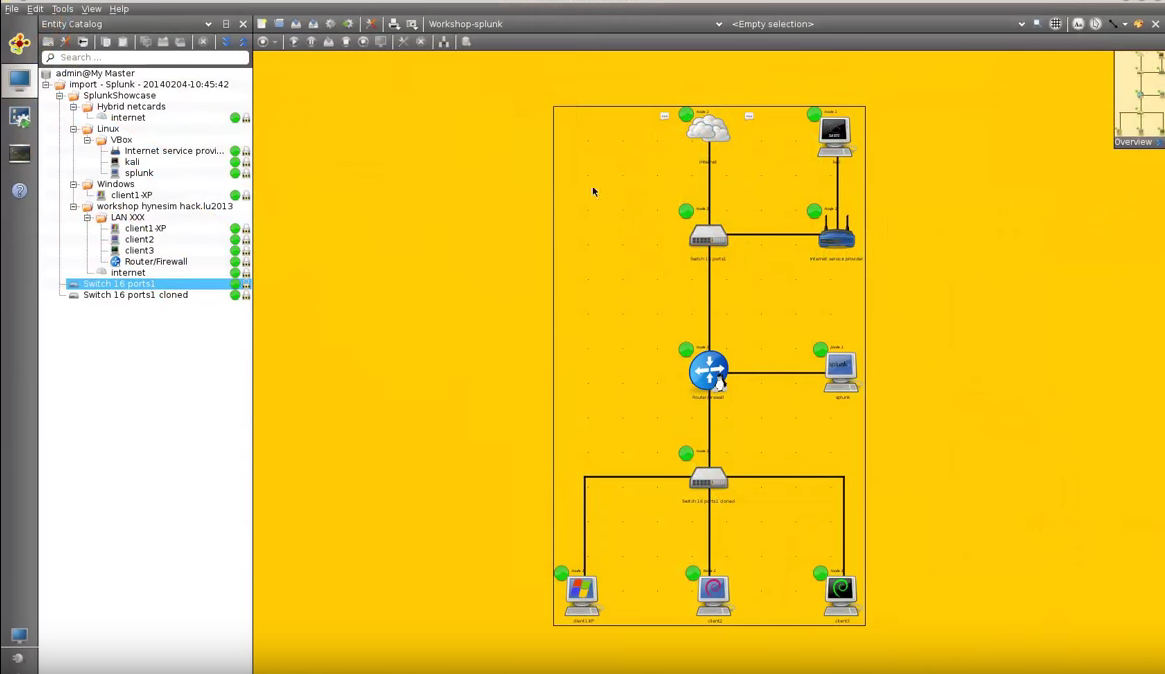
\includegraphics[width=\textwidth]{hynesim_network}
  \caption{An example of a client Hynesim interface}
\end{figure}





%%% Local Variables:
%%% mode: latex
%%% TeX-master: "../rapport_de_base"
%%% End:
